\documentclass[12pt,letterpaper]{article}
\usepackage[utf8]{inputenc}
\usepackage{amsmath}
\usepackage{amsfonts}
\usepackage{amssymb}
\usepackage{graphicx}
\usepackage{fancybox}
\usepackage{caption}
\usepackage{hyperref}
\setlength{\captionmargin}{10mm}
\renewcommand\captionfont{\it}
\renewcommand\captionlabelfont{\bf}
\hypersetup{
   pdfauthor = {Kim Siang Khaw},
	colorlinks=true, citecolor=blue, linkcolor=blue, bookmarksnumbered = true,
}
\usepackage[left=2cm,right=2cm,top=2cm,bottom=2cm]{geometry}
\author{Kim Siang Khaw}
\title{Documentation for the user interface to the Event, AMC13 and Rider Header information}

\begin{document}
\maketitle

\subsection*{Objective}
This document provides the information regarding user interface to the event, AMC13 and rider header information. All the information are stored in the art/ROOT files and standalone ROOT files with the TBranch structures in the following sections.

\subsection*{Terminology}
Several technical terms defined in this document. A run consists of multiple events. There is a maximum of 12 AMC slots per calorimeter. Each AMC slot has a Rider digitizer, and each Rider has 5 input channels.

\newpage
\section{RunHeader Class Reference}
Run header appears once for each run.

\subsection*{TLeaf members}

Below are the member variables that appear under TBranch RunHeader.

\begin{itemize}
\item ULong\_t \textbf{RunNum}
\item ULong\_t \textbf{NumOfEvent}
\item ULong\_t \textbf{NumOfAMC13Trig}
\item ULong\_t \textbf{NumOfRiderTrig}
\end{itemize}

\newpage
\section{EventHeader Class Reference}
Event header appears once for each event.

\subsection*{TLeaf members}

Below are the member variables that appear under TBranch EventHeader.

\begin{itemize}
\item ULong\_t \textbf{EventNum}
\item ULong\_t \textbf{AMC13TrigNum}
\item UChar\_t \textbf{EventType}
\item UChar\_t \textbf{NumOfAMC}
\item UChar\_t \textbf{NumOfRiderChannel}
\item struct \textbf{AMCHeader} 
    \begin{itemize}
    \item UChar\_t \textbf{AMCSlotNum}  
    \item ULong\_t  \textbf{RiderSerialNum}  
    \item ULong\_t \textbf{AMCCounter}
    \item ULong\_t \textbf{RiderTrigNum}
    \end{itemize} 
\end{itemize}

\newpage
\section{RiderChannelHeader Class Reference} 
Rider channel header appears once for each rider channel.

\subsection*{TLeaf members}

Below are the member variables that appear under TBranch RiderChannelHeader.

\begin{itemize}
\item struct \textbf{RiderChannelHeader}
      \begin{itemize}
    \item UChar\_t \textbf{AMCSlotNum}
    \item UChar\_t \textbf{RiderChannelNum}
    \item UChar\_t \textbf{FillType}
     \item ULong\_t \textbf{WaveformIndex}
    \item ULong\_t \textbf{WaveformCount}
    \item ULong\_t \textbf{TriggerNum}
    \item UInt\_t \textbf{WaveformLength}
    \end{itemize}
\end{itemize}

\newpage
\appendix

\section{Data Formats}

This section compiles all the available header data formats. Please refer to \url{http://gm2-docdb.fnal.gov:8080/cgi-bin/ShowDocument?docid=3409} for more details.

\begin{figure}[htbp]
\centering
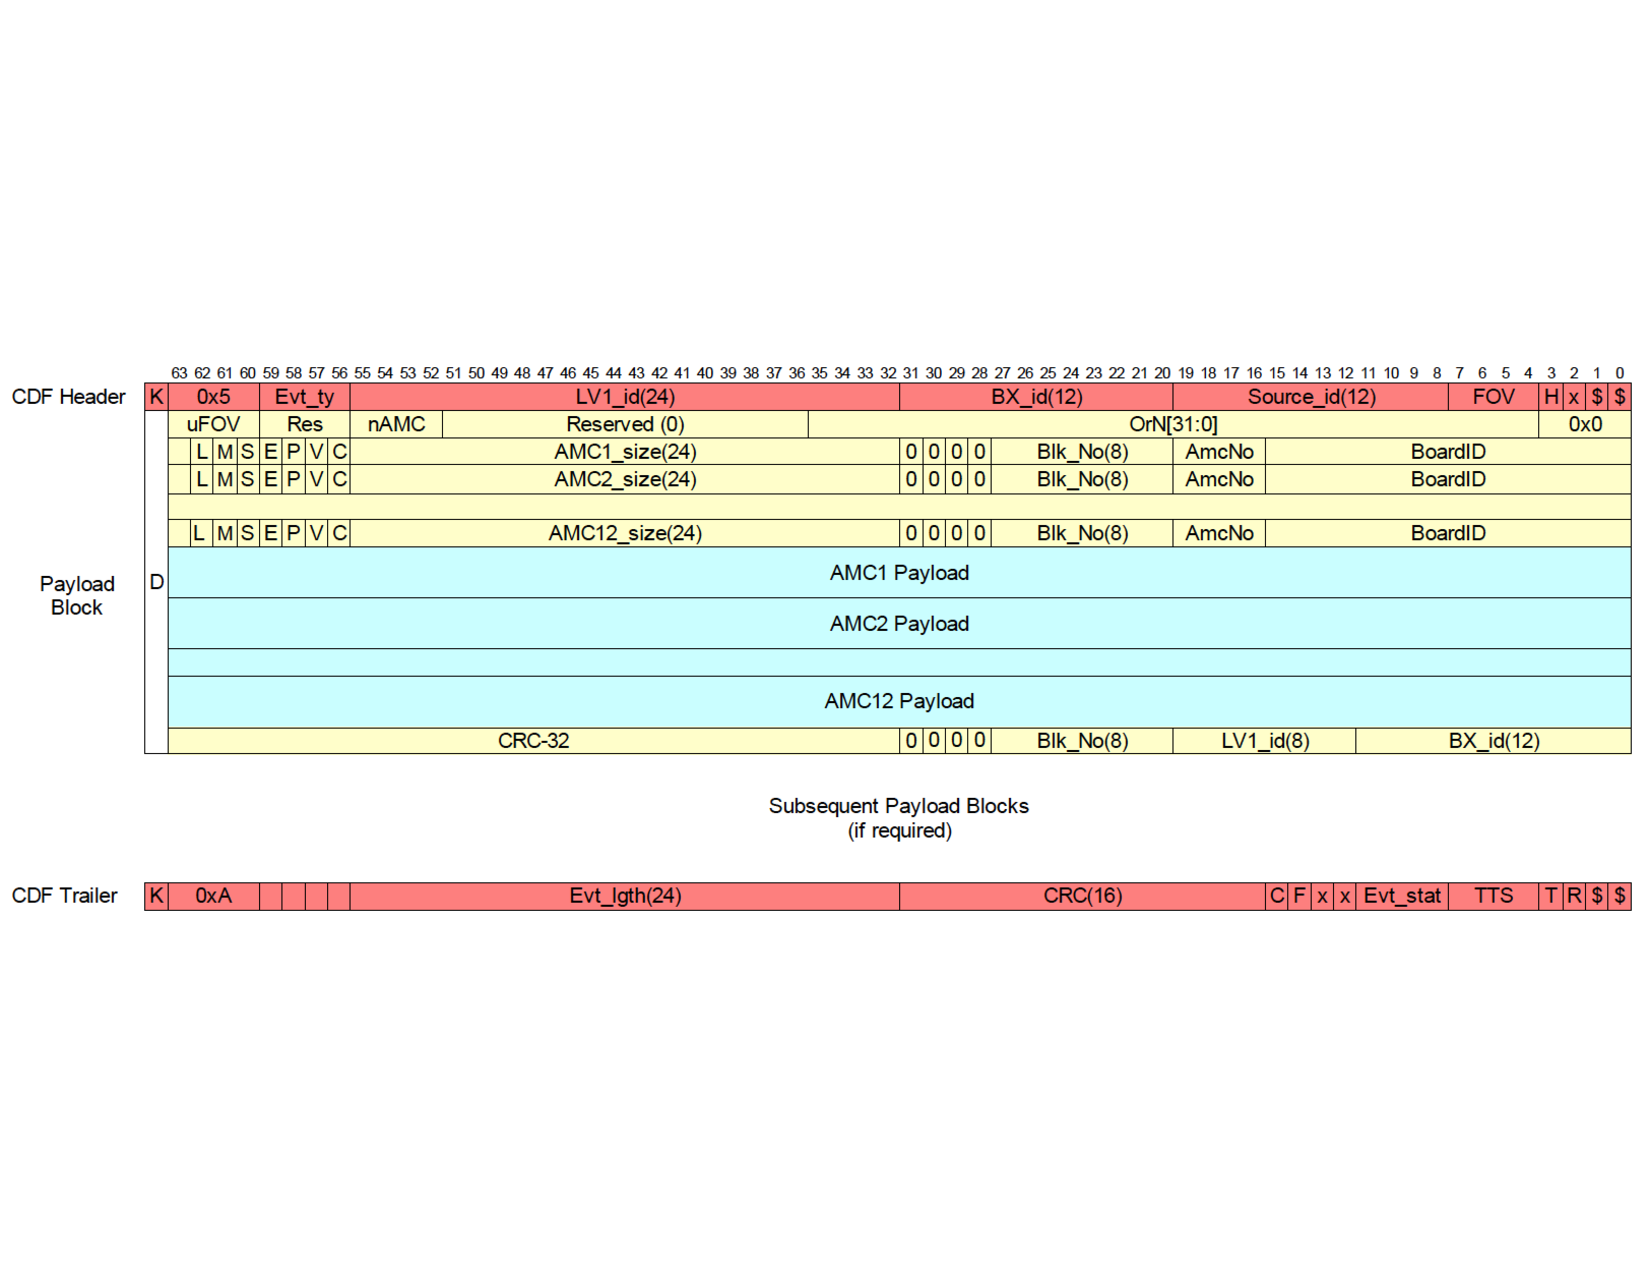
\includegraphics[trim=0cm 6cm 0cm 6cm ,width=0.95\textwidth]{pics/AMC13Header}
\caption{AMC13 to DAQ data format.}
\end{figure}

\begin{figure}[htbp]
\centering
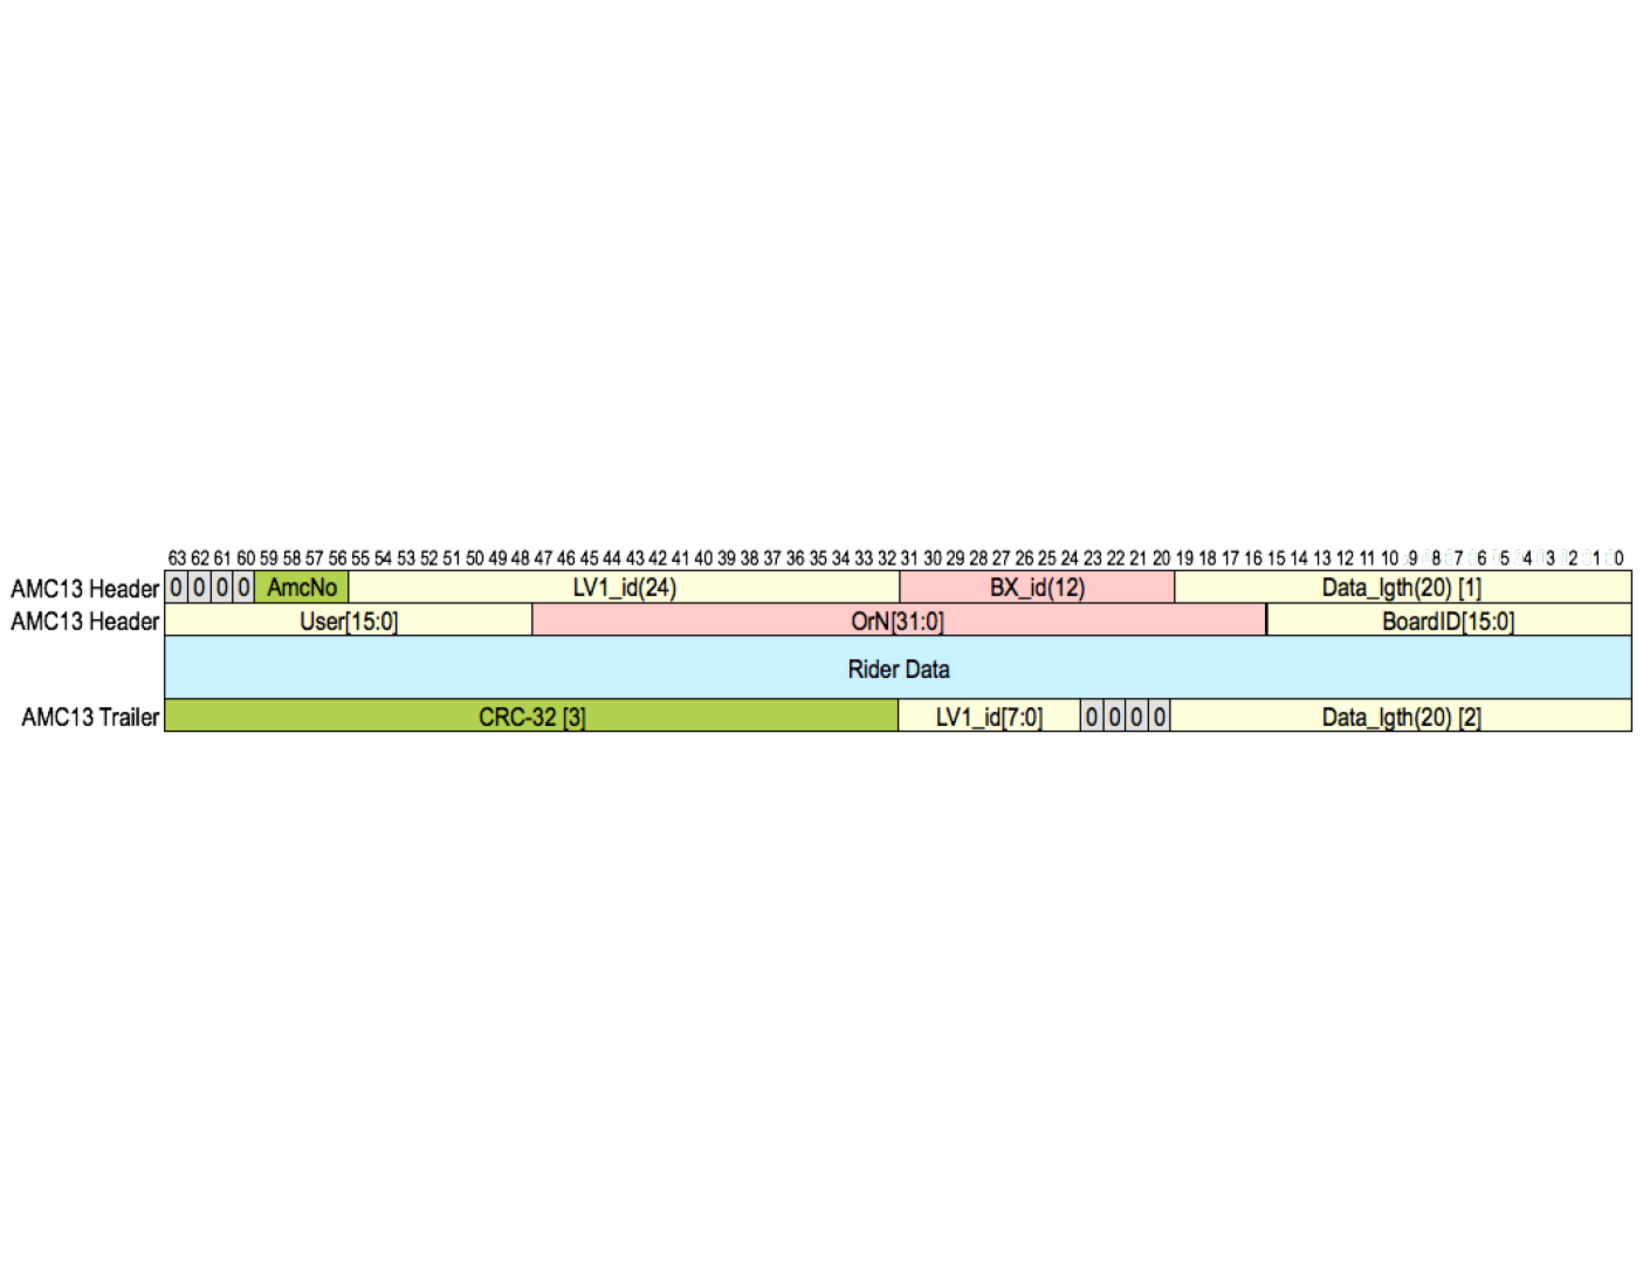
\includegraphics[trim=0cm 9.5cm 0cm 9.5cm ,width=0.95\textwidth]{pics/RiderToAMC13Header}
\caption{Rider to AMC13 data format.}
\end{figure}

%trim left bottom right top
\begin{figure}[htbp]
\centering
%\fbox{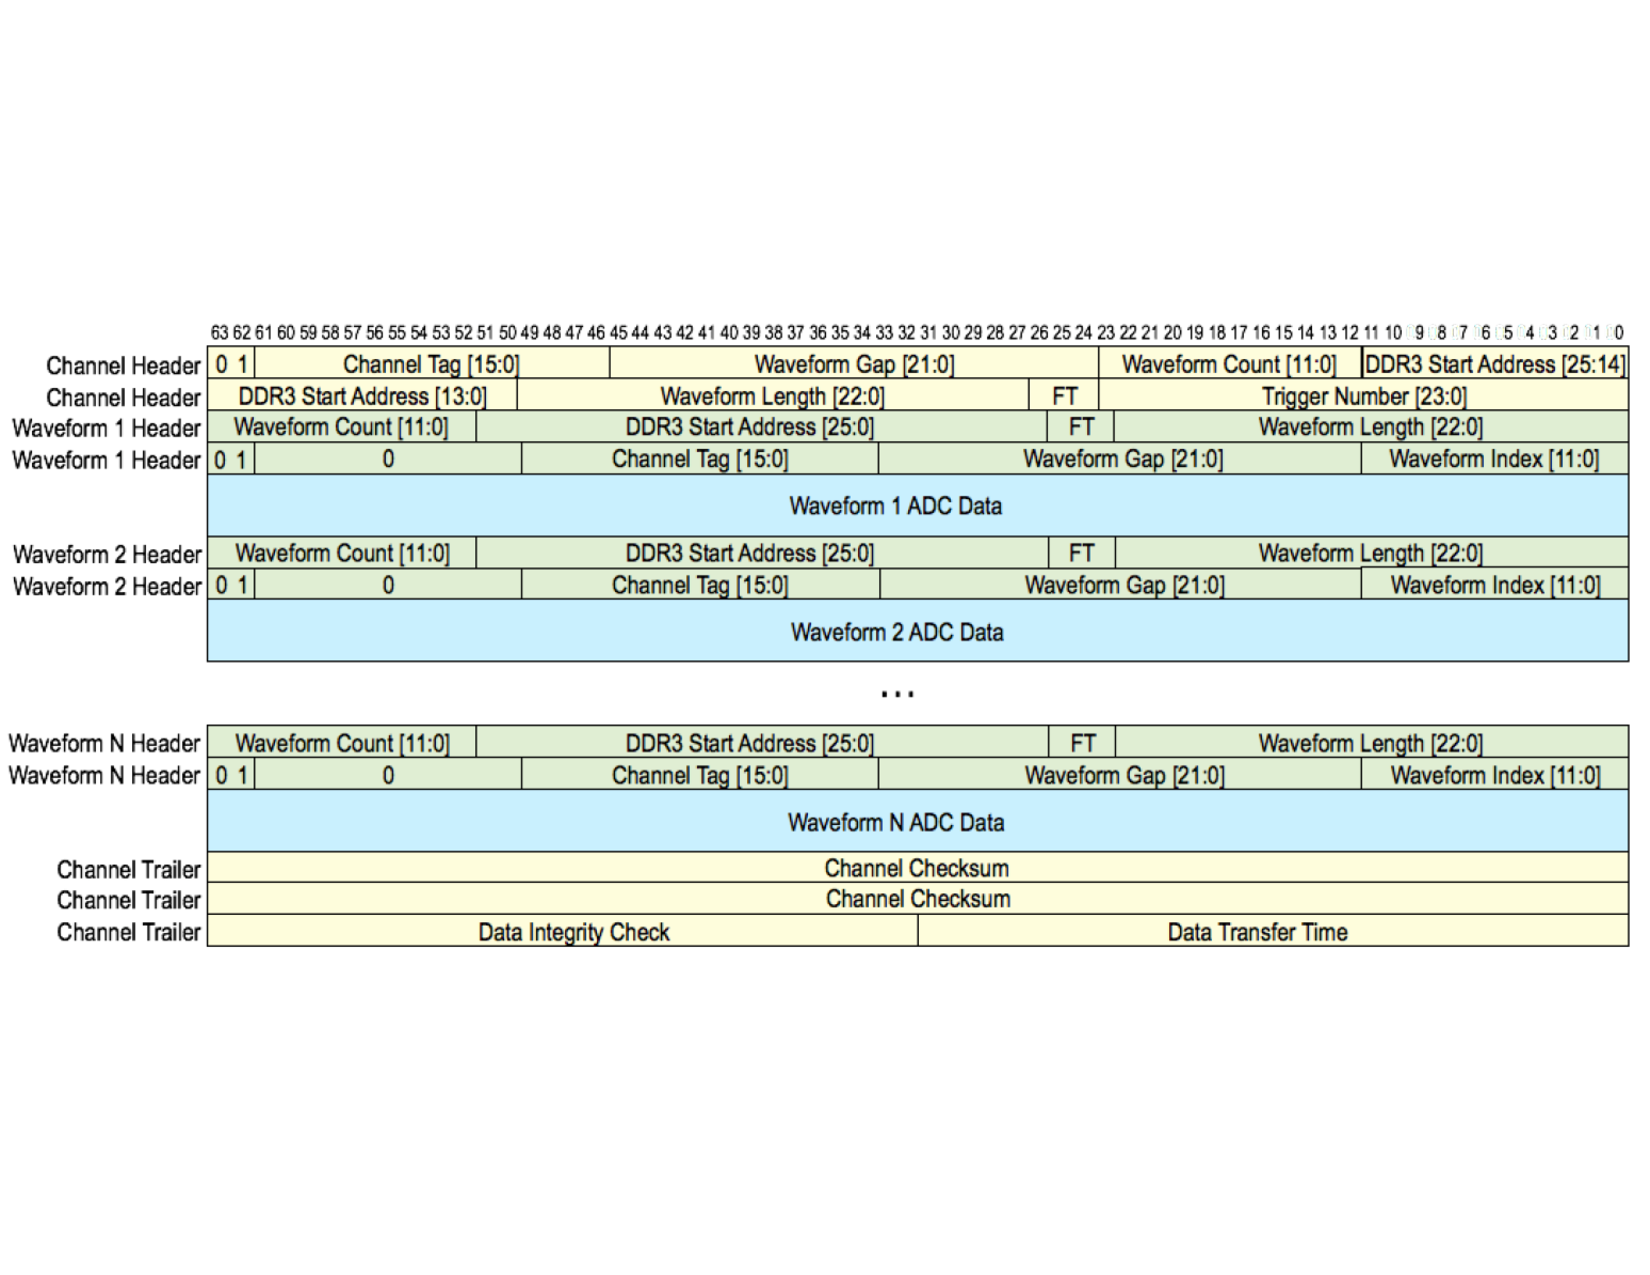
\includegraphics[trim=0cm 5.5cm 0cm 5.5cm ,width=0.9\textwidth]{pics/RiderChannelHeader}} guide line for trimming
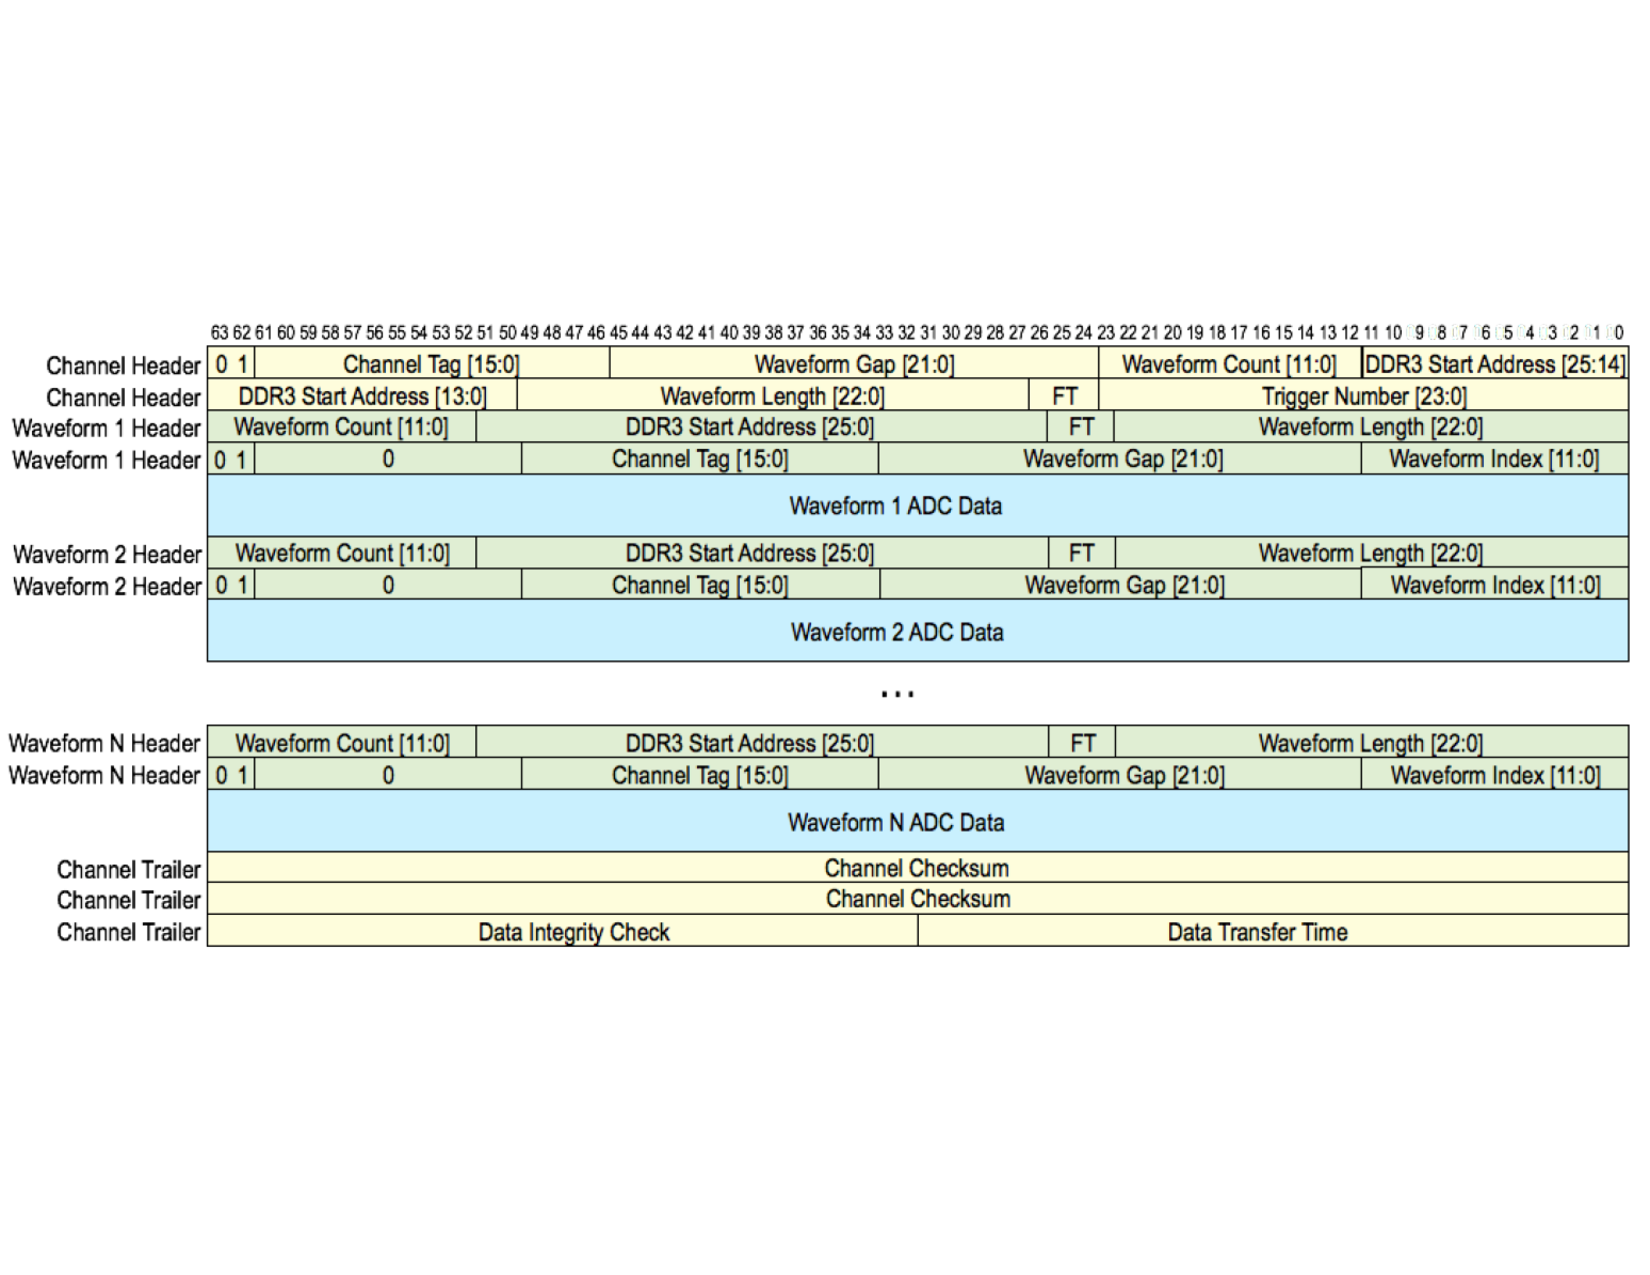
\includegraphics[trim=0cm 5.5cm 0cm 5.5cm ,width=0.95\textwidth]{pics/RiderChannelHeader}
\caption{Rider Channel data format.}
\end{figure}

\begin{figure}[htbp]
\centering
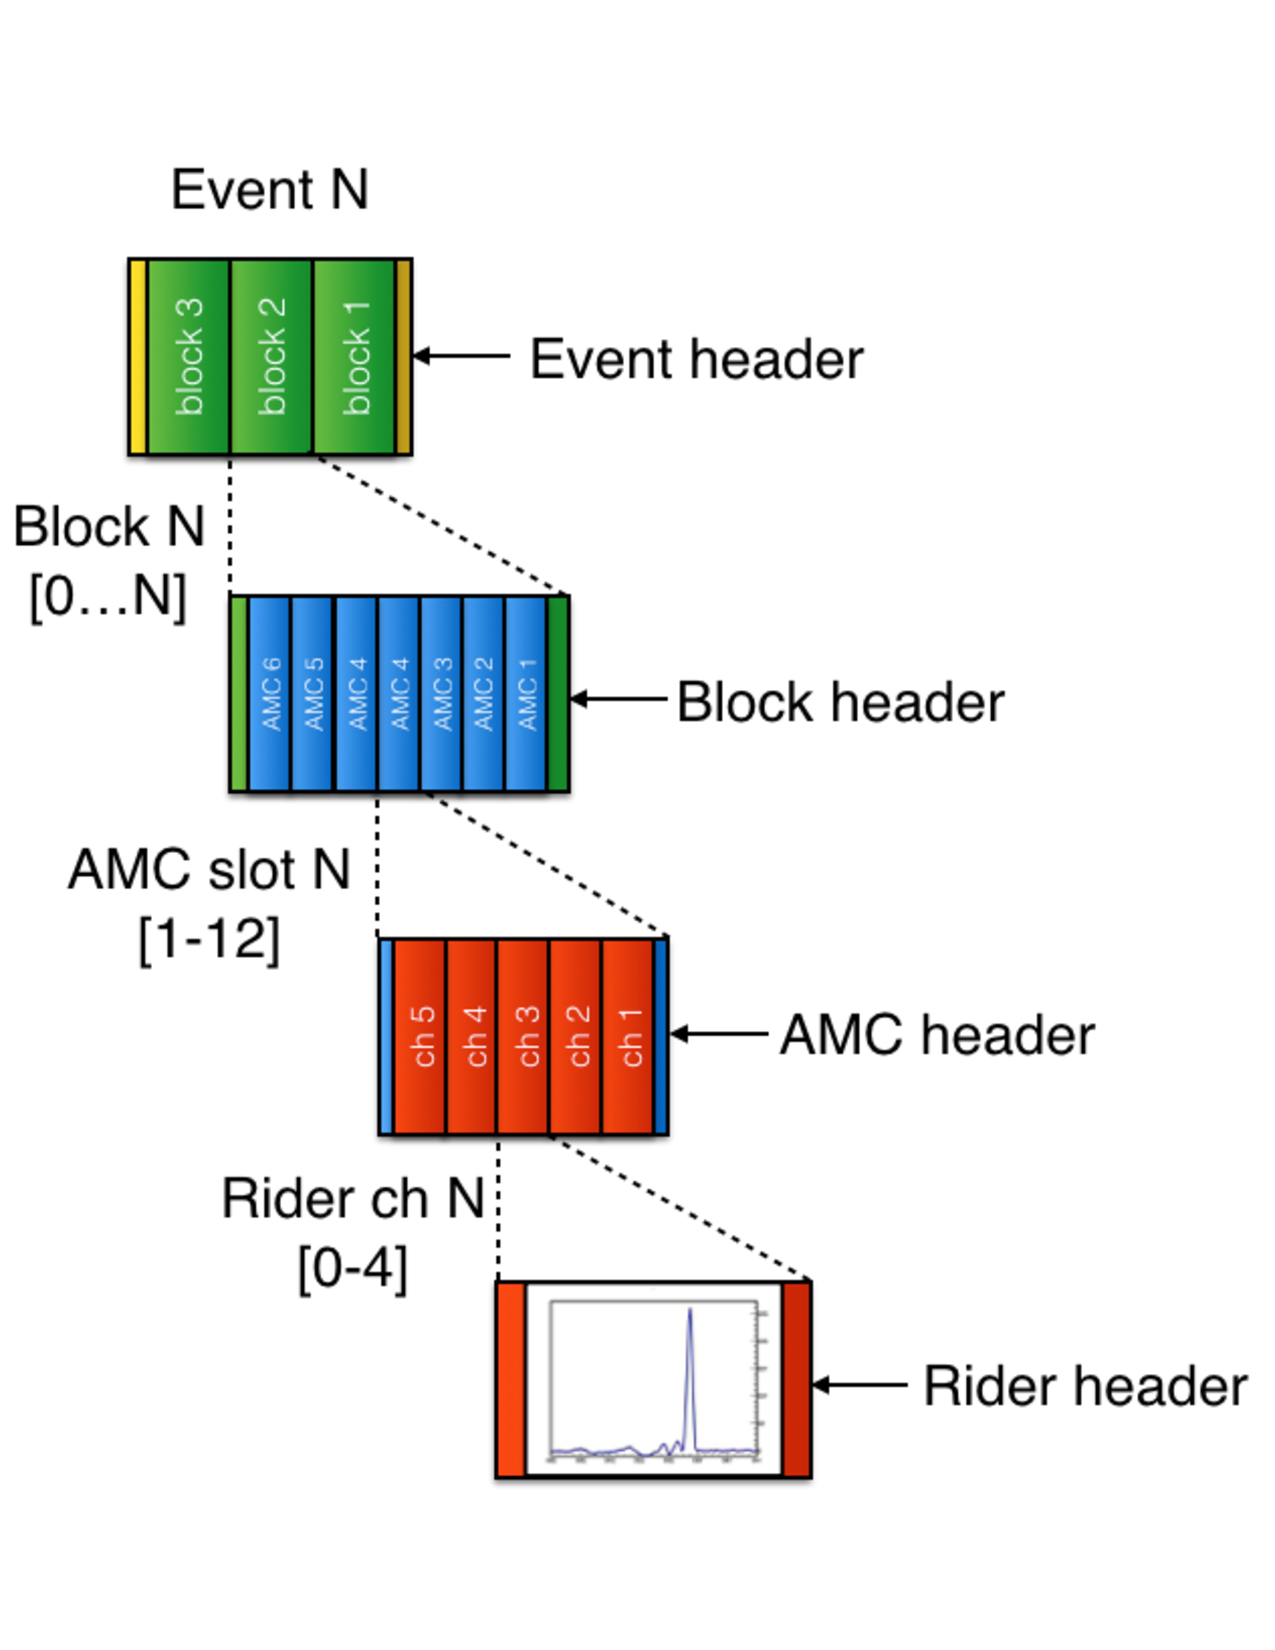
\includegraphics[width=0.9\textwidth]{pics/AllHeaders}
\caption{Per event data format}
\end{figure}
\end{document}